\subsection{Performance analysis of the algorithms}
\label{performance-analysys}
We said in~\ref{sort-fram} that sorting a data set is a computation described by a \textit{5-tuple} $\langle n$, $M$, $s$, $\Lambda$, $\sigma \rangle$, with $n$ the parallelism degree, $M$ the size of the data set, $s$ a seed for generating the data set, $\Lambda$ the algorithm and $\sigma$ a set of parameters depending on $\Lambda$. In reality, $\sigma$ is significative just for some algorithms; for instance, it can specify the \textit{stencil} (communication pattern) for the processes of a parallel algorithm or the value of ''\textit{K}'' in algorithms like \textit{K-way mergesort}. For each $\Lambda$, we will run single-shot computations (that is, there are not streams of data sets to sort) by varying $n$, $M$, $s$. Initially, $\sigma$ will be fixed for every computations. It is a convention that we will refer to \textit{small}, \textit{large} or \textit{huge} data sets for sizes that are respectively a few MBs, hundreads of MBs and (at least) GBs. 

In order to analyze the performance of the algorithms from different perspective (e.g.: scalability of the specific algorithm, comparison of the time completion required by different algorithms to sort a specific data set and so on) we are going to show different types of graphics. Each graphic is defined by a 3-tuple $\langle x, y, plot \rangle $, where $x$ is the variable on the X axis, $y$ the variable on the Y axis and $plot$ a parameter that identifies a specific shape of that graphic. In particular, given $T$ the time completion of a computation, we will focus on the following graphics:
\begin{enumerate}
\item fixed $M$, a graphic $\langle n, T, \Lambda \rangle $ is necessary to see which is \textit{the ''best'' algorithm} for sorting a data set of a certain $M$ on a specific architecture. Here, we refer to the ''best'' algorithm(s) as the one(s) that is able either to sort faster a specific data set, to scale better or a combination of them. 
\item fixed $\Lambda$, a graphic $\langle n, T, M \rangle$ is useful to see the \textit{scalability} of $\Lambda$ on a specific architecture. Different shapes shows the scalability of $\Lambda$ for different sizes of the data set.
\item fixed $\Lambda$, a graphic $\langle M, T, n \rangle$ to show (as before) the behaviour of $\Lambda$ on a specific architecture, but from a different perspective. 
\item a graphic $\langle M, T, \Lambda \rangle$ to understand which algorithm \textit{should} be used if the target architecture allowed a parallelism degree of at most $n$. These graphics could be used as ''experimental cost models'', in sense that in principle they could predict the performance of a Sorting Algorithm on such architectures that are ''similar'' to our target architectures. Here, ''similar'' refers mainly to CPUs, memory hierarchies, I/O subsystem, interconnection structure.  
\end{enumerate}

The parameters of the computations will take the following values:
\begin{itemize}
\item $\Lambda \in \lbrace$Sequentialsort, Bitonicsort, Samplesort, Bucketsort, Mergesort, Quicksort, K-Way Mergesort, Load-Balanced Mergesort, Load-Balanced Multi-Way Mergesort$\rbrace$;
\item $n \in \lbrace$1, 2, 4, 8, 16, 32, 64, 128, 256$\rbrace$; notice that the maximum value that $n$ can take depends on the specific architecture. 
\item $M \in \lbrace 2^{10 + i} : i = 0, ..., 25\rbrace$ elements (integers). So $M$ takes values from a few kilobytes to tens of gigabytes (recall that each integers is usually represented through 4 bytes).
\end{itemize} 

For each target architecture, first we will focus on analyzing the scalability of each Sorting Algorithms (graphics 2, 3). Then, we will compare them by fixing the size of the data set and showing which algorithm sorts it faster, for different parallelism degrees (graphic 1). Finally, we will show and explain which is the best algorithm for our target architectures. 

\subsubsection{Pianosa}
On this architecture, due to the lack of space on disks, we will be able to test Sorting Algorithms for data sets of size at most 4GB, namely 1G integers. Further, given the results of tests shown in~\ref{test-env-pianosa}, the size of the communication buffer of the DAL layer has been set to 10MB. 

\paragraph{Scalability of Sorting Algorithms}
%Figure~\ref{large-tc} shows the completion time for sorting large data sets. One thing is clearly visible: for parallelism degrees up to 8, sequential $qsort$ even outperforms almost all the algorithms; for parallelism degree 16 some algorithms improve a little the completion time ($Samplesort$, $Bucketsort$, $Mergesort$, $Load$-$Balanced$ $Multi$-$Way$ $Mergesort$), but anyway it keeps to be very close (same order magnitude) to the one of $qsort$. However, this result is not really surprising. Indeed, as we told in advance, we must take care of the following features:
%\begin{itemize}
%\item the computation performed on each element of the data set has fine grain;
%\item the whole data set is of the order of MBs. In the best case, changing the parallelism degree from $2$ to $4$ (or at most from $4$ to $8$) and assuming a data set size of $400$ MB, we notice that almost all parallel algorithms significatively (but not ideally) improve the completion time. This is because each process can work on a portion of data that is still roughly a hundred of MBs. In all other cases, each process works on very smaller portion of data, so the parallelization, given that the computation on each element has fine grain, is not so useful. 
%\item the cost and the number of communications that, as we saw in~\ref{test-env-pianosa}, may impact the completion time. We will further investigate and detail the impact of communications in the final version of the report.
%\end{itemize}
%These consideration aims at justifying the non-ideal scalability of the algorithms. We hope that for huge data sets we will be able to improve these results by increasing the time spent by each process on the sequential computation, hoping that it will be relatively larger than the one spent in communications. Surely, at least the difference between the time completion of parallel algorithms and the one of sequential qsort will become significant.

If the data set is small (i.e. of size up to 64MB) there is not any Sorting Algorithms that scales. Even worse, if we plotted the same shapes of Figure~\ref{NxTxM} on a logarithmic scale, we would notice that by increasing the parallelism degree we would obtain an increase of the Time Completion too. In reality, this behaviour is not surprising. The cost of \textit{Sequentialsort} for small data sets varies between a few seconds and tens of milliseconds, that is the same order magnitude of $T\_send( KB )$ (see~\ref{test-env-pianosa} for more details). This means that the cost of communications between processes has a fundamental impact on the final performance of Sorting Algorithms. Therefore, from a qualitative point of view, the higher the parallelism degree, the higher both the number of communications and the overall time spent in sending datas, so higher is even the overhead introduced by the parallelization. Our conclusion is that on Pianosa, for small data sets, the best choice is a sequential sorting algorithm (like the ANSI \textit{qsort}).

Things are a little bit different when the data set is large, namely when its size is between 128MB and 512MB. Figure~\ref{NxTxM} clearly shows that there is not any algorithm that scales. Bucketsort and Samplesort have a little improvement passing from $n=2$ to $n=4$, but nothing extraordinary. However, if the data set is of 512MB, the parallelization is useful to lower the Time Completion with respect to the one of \textit{Sequentialsort}. Figure~\ref{sequential-pianosa} shows that, for sorting 512 MB, \textit{Sequentialsort} takes roughly 400s, while all Sorting Algorithms, except Quicksort, are able to lower it up to roughly 200s with just $n=4$. Unfortunately, we do not obtain any further improve neither moving from $n=4$ to $n=8$ nor considering a smaller data size (with just $M=256MB$ the parallelizzation gain is not significative). Reasons are quite obvious. From one hand, if we increase the parallelism degree the negative impact of communications is greater than the gain coming from having more computational units (working on smaller partitions).  From the other hand, $M=512MB$ means a jump to an important computational grain: indeed, moving from $n=2$ to $n=4$ guarantees processes to work with a partition of the data set that is still significative; this explains why some Sorting Algorithms shows a gain in terms of Time Completion within this range of processes. If we further increase $n$ up to $16$, processes have to work on smaller partitions, which let the parallelization in some sense useless.



\begin{figure}[!ht]
	\begin{center}
		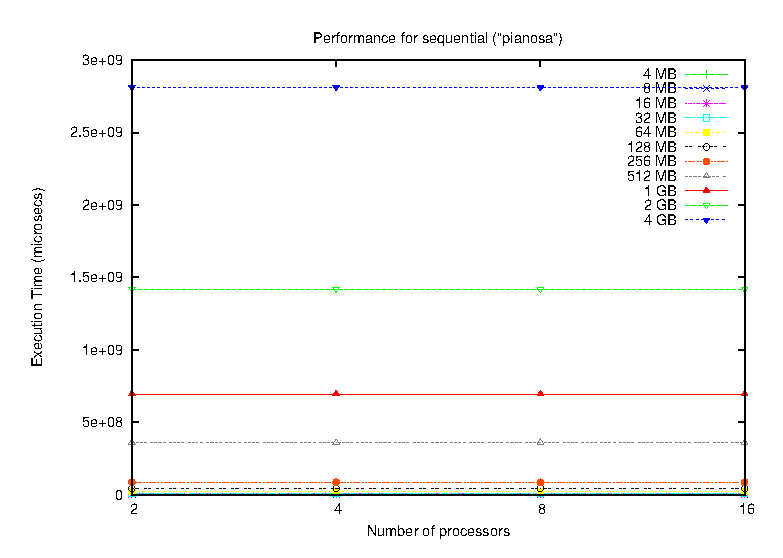
\includegraphics[scale=0.6]{plots/test_01_pianosa/NxTxM/sequential_pianosa_NxTxM}
	\end{center}
  	\caption{Completion Time on Pianosa for the Sequentialsort.}
  	\label{sequential-pianosa}
\end{figure}

\begin{figure}[h]
	\centering
	\subfloat[Quicksort.]{\label{large-sequential}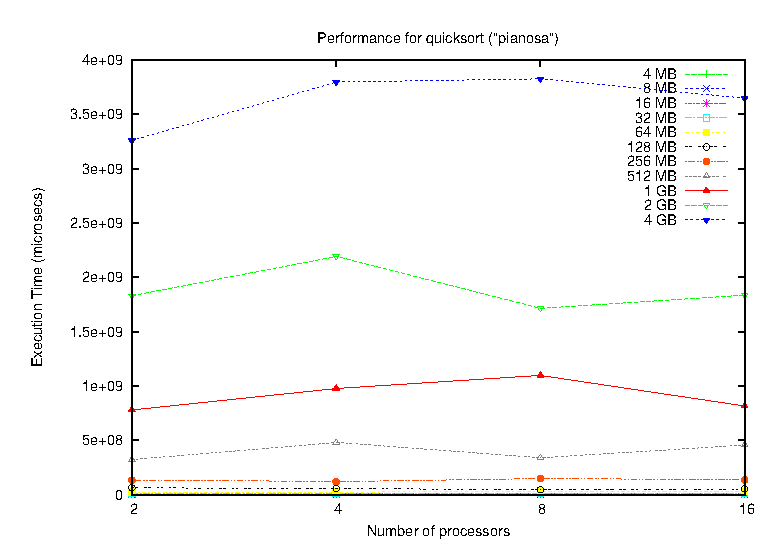
\includegraphics[width=0.4\textwidth]{plots/test_01_pianosa/NxTxM/quicksort_pianosa_NxTxM}} 
	\hspace*{20pt}	
  	\subfloat[Bitonicsort.]{\label{large-bitonicsort}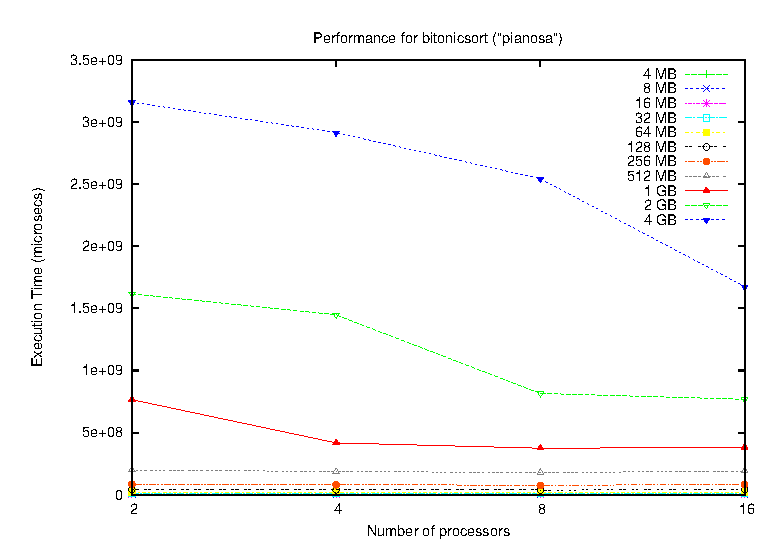
\includegraphics[width=0.4\textwidth]{plots/test_01_pianosa/NxTxM/bitonicsort_pianosa_NxTxM}} 
  		
	\centering
	\subfloat[Bucketsort.]{\label{large-bucketsort}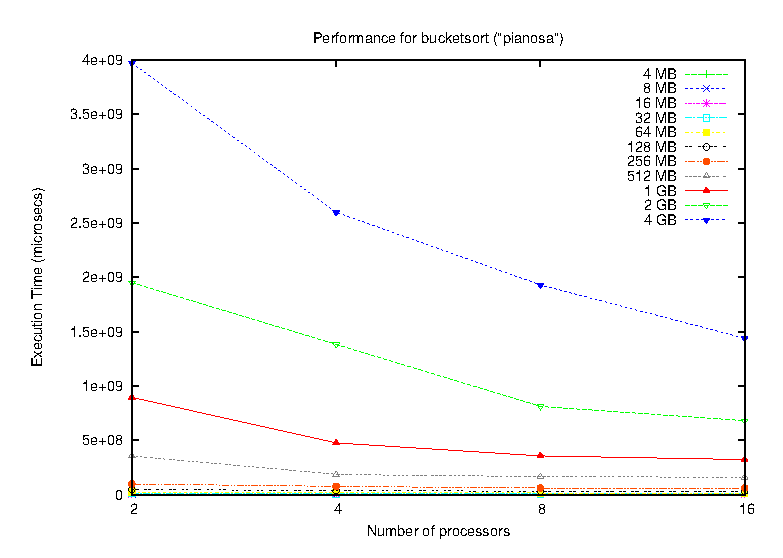
\includegraphics[width=0.4\textwidth]{plots/test_01_pianosa/NxTxM/bucketsort_pianosa_NxTxM}} 
  	\hspace*{20pt}
  	\subfloat[Samplesort.]{\label{large-samplesort}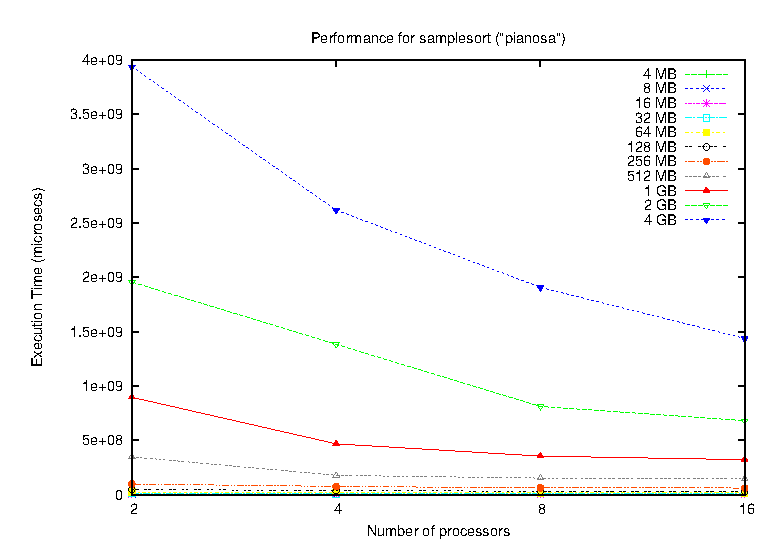
\includegraphics[width=0.4\textwidth]{plots/test_01_pianosa/NxTxM/samplesort_pianosa_NxTxM}} 
	
	\centering
  	\subfloat[Mergesort.]{\label{large-mergesort}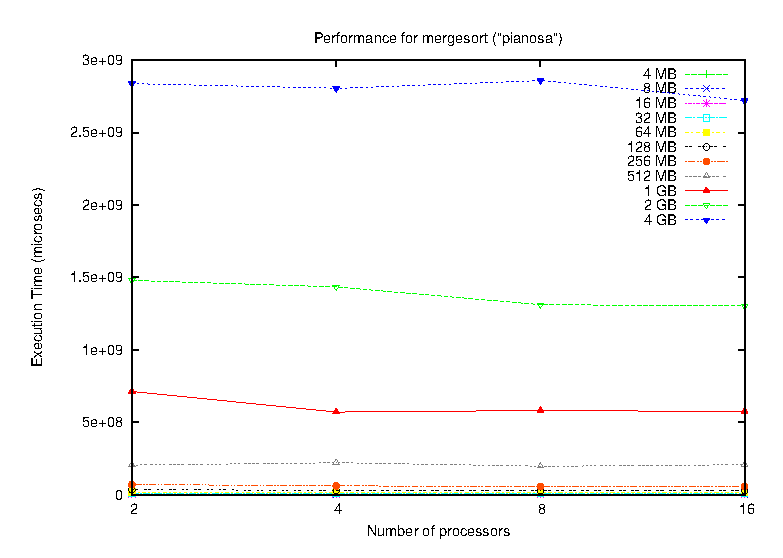
\includegraphics[width=0.4\textwidth]{plots/test_01_pianosa/NxTxM/mergesort_pianosa_NxTxM}}   
  	\hspace*{20pt}  
  	\subfloat[4-Way Mergesort.]{\label{large-kmerge}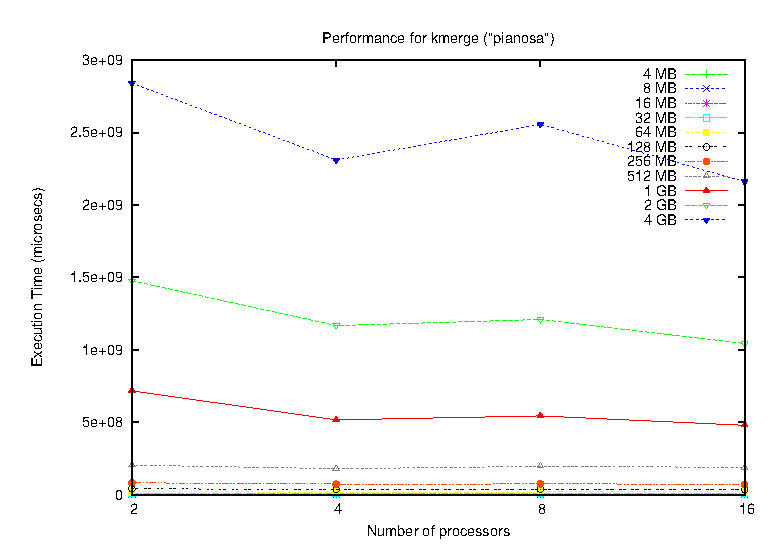
\includegraphics[width=0.4\textwidth]{plots/test_01_pianosa/NxTxM/kmerge_pianosa_NxTxM}} 
	
	\centering
  	\subfloat[Load-Balanced Mergesort.]{\label{large-lbmergesort}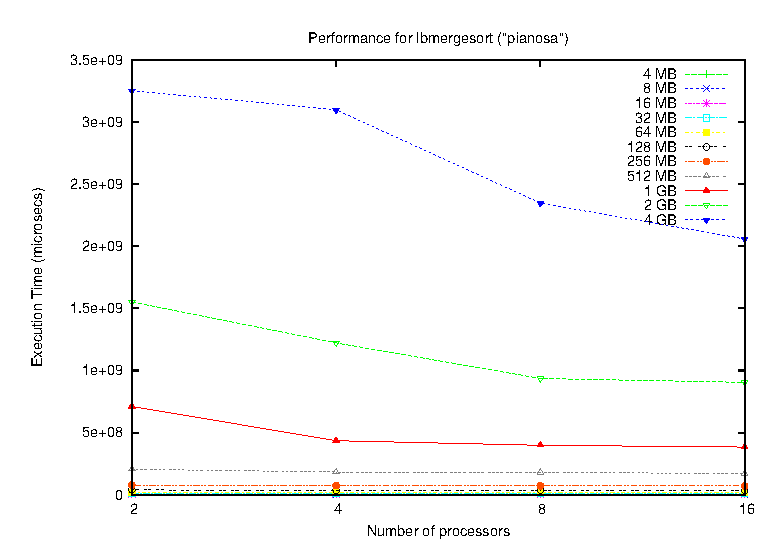
\includegraphics[width=0.4\textwidth]{plots/test_01_pianosa/NxTxM/lbmergesort_pianosa_NxTxM}} 
  	\hspace*{20pt}  
  	\subfloat[Load-Balanced Multi-Way Mergesort.]{\label{large-lbkmergesort}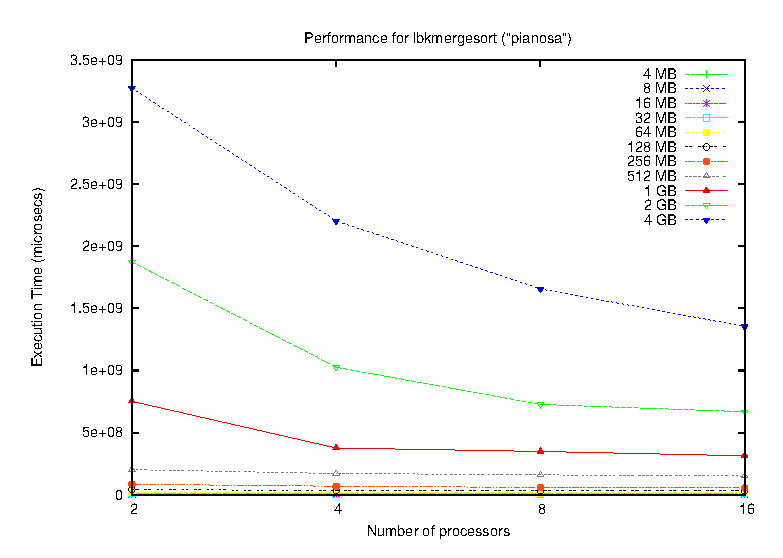
\includegraphics[width=0.4\textwidth]{plots/test_01_pianosa/NxTxM/lbkmergesort_pianosa_NxTxM}} 
  	
	\caption{Time Completion of Sorting Algorithms by varying the parallelism degree. Each shape on a graphic represents the Time Completion of a certain Sorting Algorithm for a data set of specific size.}
	\label{NxTxM}
\end{figure}
 
\begin{figure}[!ht]
	\centering
	\subfloat[Quicksort.]{\label{large-sequential}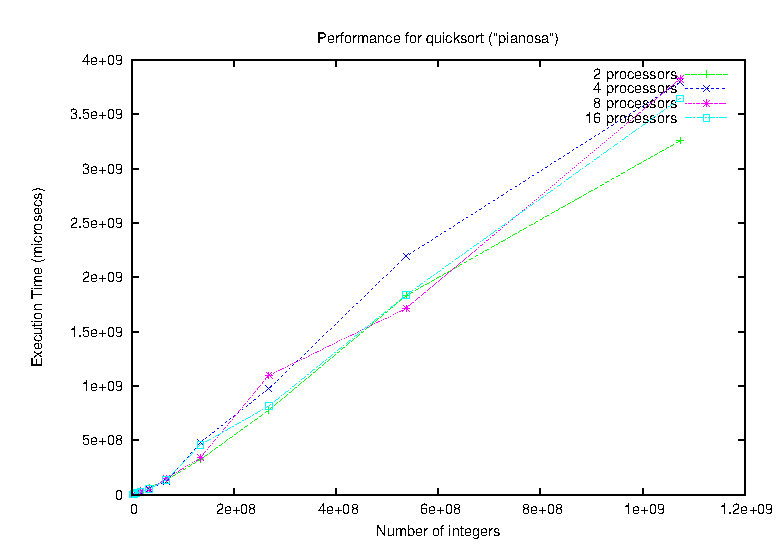
\includegraphics[width=0.4\textwidth]{plots/test_01_pianosa/MxTxN/quicksort_pianosa_MxTxN}} 
	\hspace*{20pt}	
  	\subfloat[Bitonicsort.]{\label{large-bitonicsort}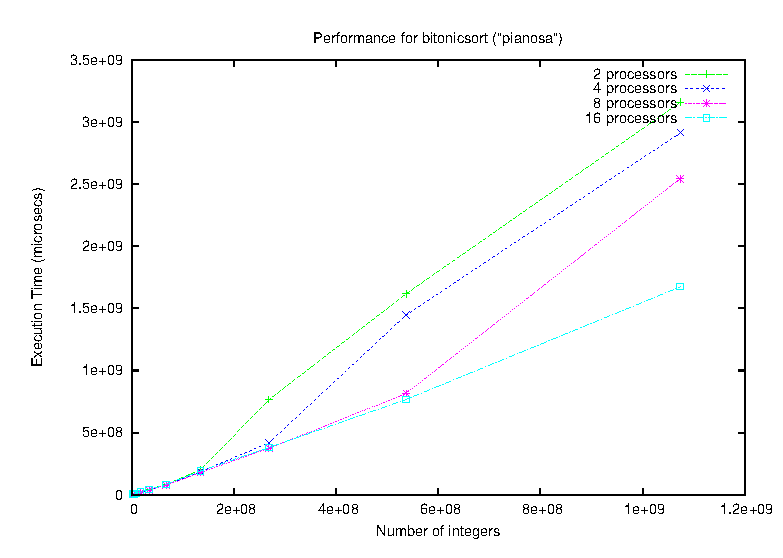
\includegraphics[width=0.4\textwidth]{plots/test_01_pianosa/MxTxN/bitonicsort_pianosa_MxTxN}} 
  		
	\centering
	\subfloat[Bucketsort.]{\label{large-bucketsort}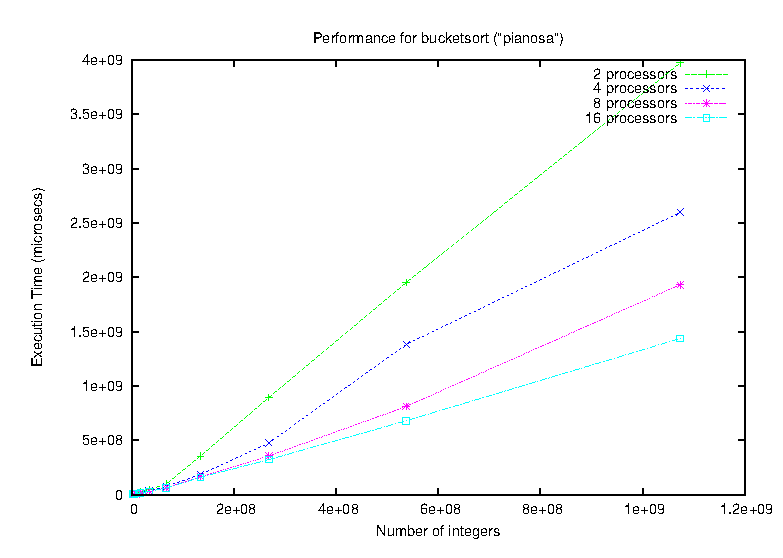
\includegraphics[width=0.4\textwidth]{plots/test_01_pianosa/MxTxN/bucketsort_pianosa_MxTxN}} 
  	\hspace*{20pt}
  	\subfloat[Samplesort.]{\label{large-samplesort}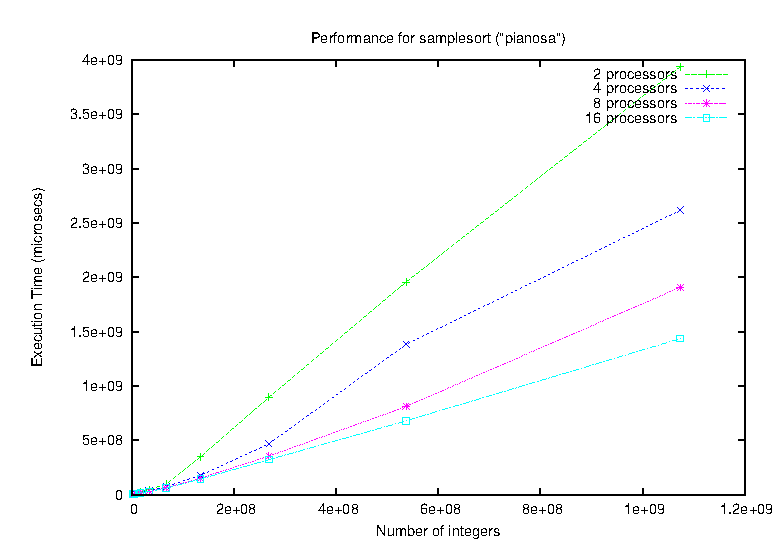
\includegraphics[width=0.4\textwidth]{plots/test_01_pianosa/MxTxN/samplesort_pianosa_MxTxN}} 
	
	\centering
  	\subfloat[Mergesort.]{\label{large-mergesort}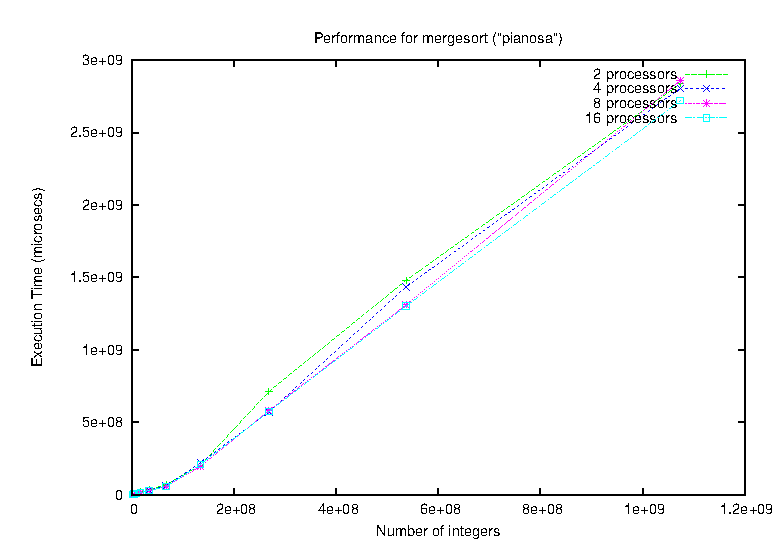
\includegraphics[width=0.4\textwidth]{plots/test_01_pianosa/MxTxN/mergesort_pianosa_MxTxN}}   
  	\hspace*{20pt}  
  	\subfloat[4-Way Mergesort.]{\label{large-kmerge}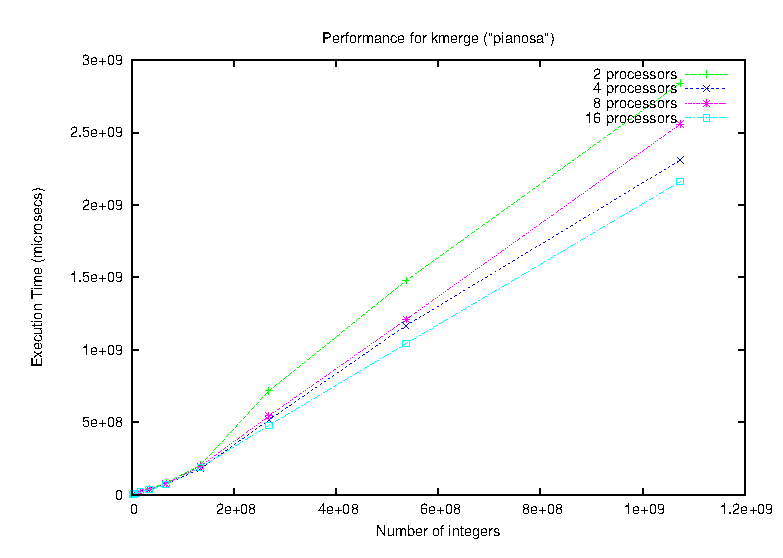
\includegraphics[width=0.4\textwidth]{plots/test_01_pianosa/MxTxN/kmerge_pianosa_MxTxN}} 
	
	\centering
  	\subfloat[Load-Balanced Mergesort.]{\label{large-lbmergesort}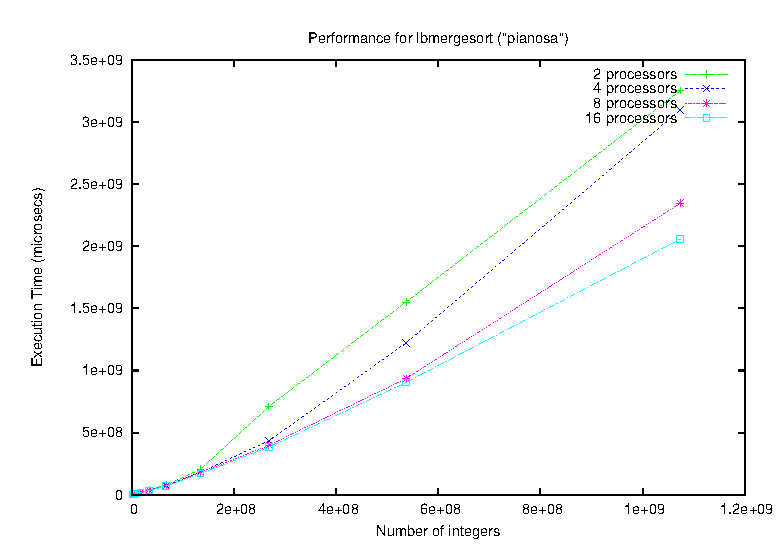
\includegraphics[width=0.4\textwidth]{plots/test_01_pianosa/MxTxN/lbmergesort_pianosa_MxTxN}} 
  	\hspace*{20pt}  
  	\subfloat[Load-Balanced Multi-Way Mergesort.]{\label{large-lbkmergesort}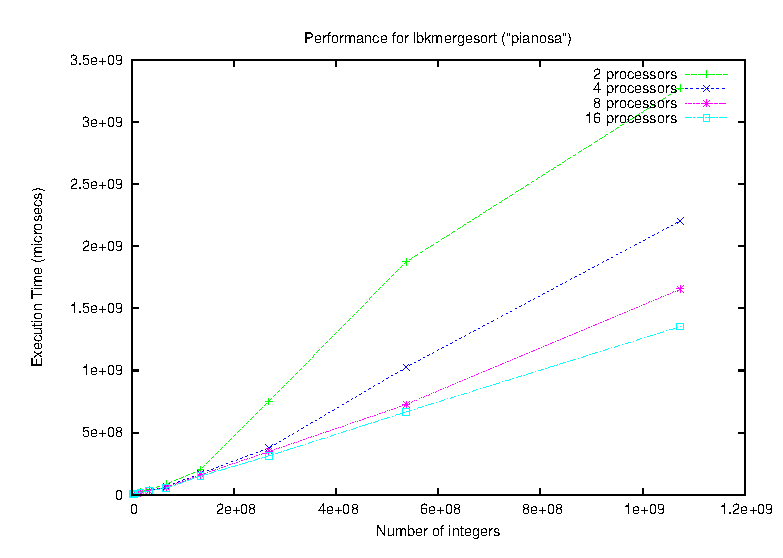
\includegraphics[width=0.4\textwidth]{plots/test_01_pianosa/MxTxN/lbkmergesort_pianosa_MxTxN}} 
  	
	\caption{Time Completion of Sorting Algorithms for increasing sizes of the data set. }
	\label{MxTxN}
\end{figure} 
 
 
\paragraph{Comparison between Sorting Algorithms}

\begin{figure}[!ht]
	\ContinuedFloat
	\centering
	\subfloat[Data set of 1M integers.]{\label{large-sequential}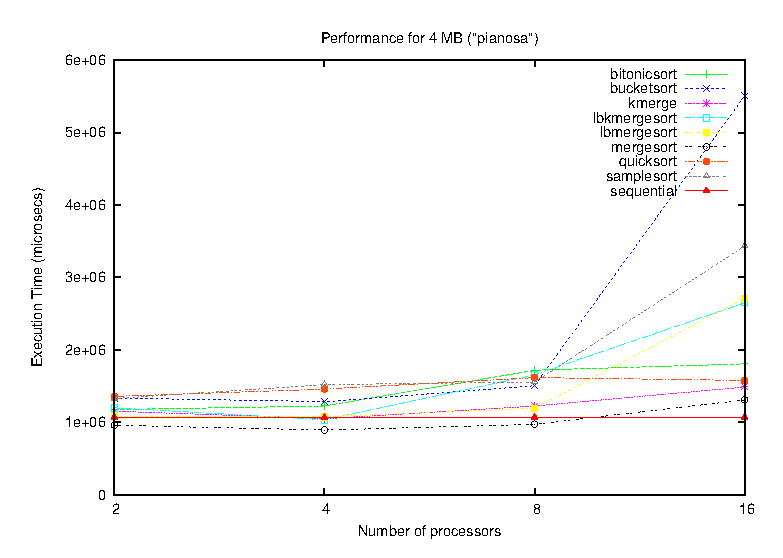
\includegraphics[width=0.4\textwidth]{plots/test_01_pianosa/NxTxA/M1048576_pianosa_NxTxA}} 
	\hspace*{20pt}	
  	\subfloat[Data set of 2M integers.]{\label{large-bitonicsort}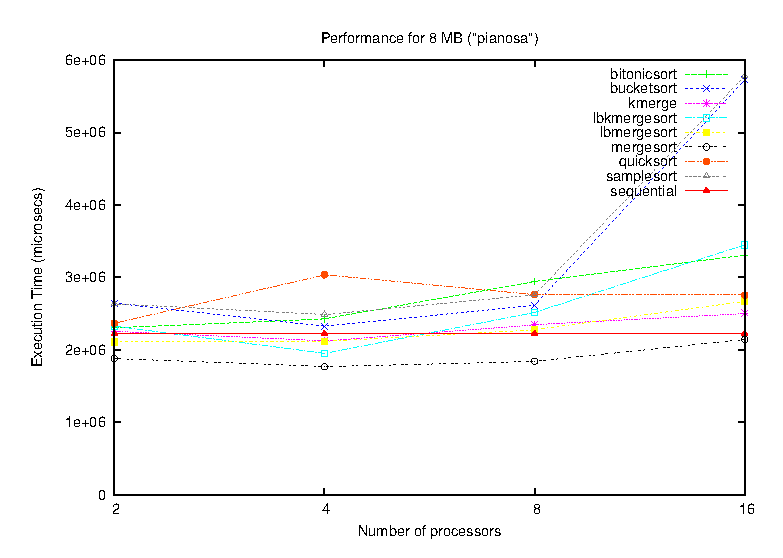
\includegraphics[width=0.4\textwidth]{plots/test_01_pianosa/NxTxA/M2097152_pianosa_NxTxA}} 
  		
	\centering
	\subfloat[Data set of 4M integers.]{\label{large-bucketsort}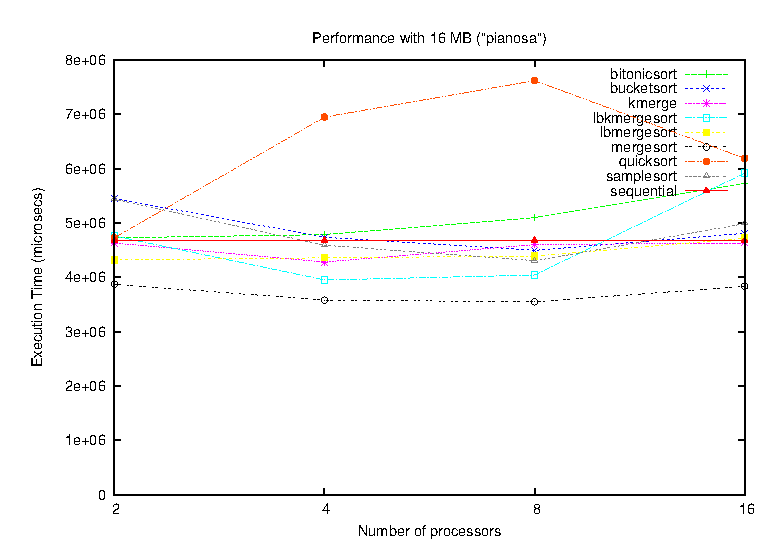
\includegraphics[width=0.4\textwidth]{plots/test_01_pianosa/NxTxA/M4194304_pianosa_NxTxA}} 
  	\hspace*{20pt}
  	\subfloat[Data set of 8M integers.]{\label{large-samplesort}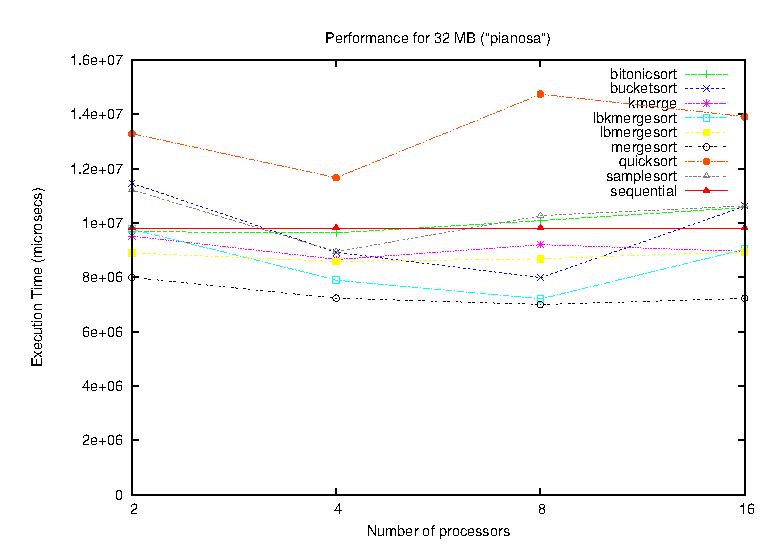
\includegraphics[width=0.4\textwidth]{plots/test_01_pianosa/NxTxA/M8388608_pianosa_NxTxA}} 
	
	\centering
  	\subfloat[Data set of 16M integers.]{\label{large-mergesort}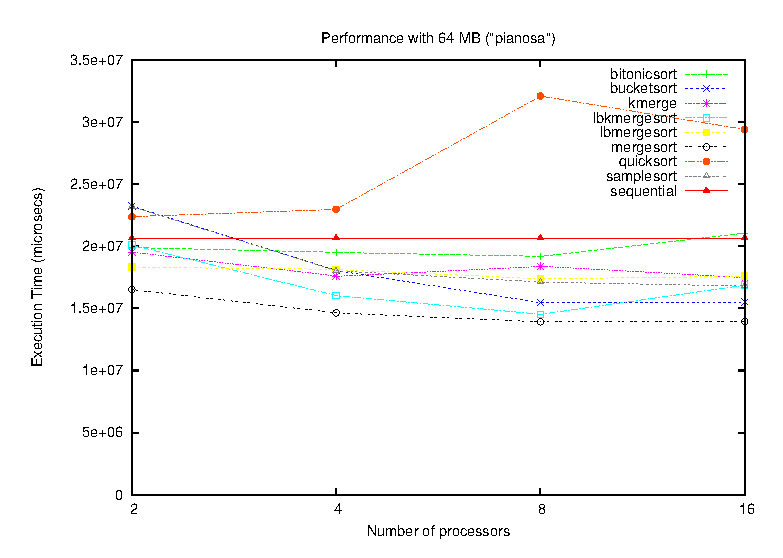
\includegraphics[width=0.4\textwidth]{plots/test_01_pianosa/NxTxA/M16777216_pianosa_NxTxA}}   
  	\hspace*{20pt}  
  	\subfloat[Data set of 32M integers.]{\label{large-kmerge}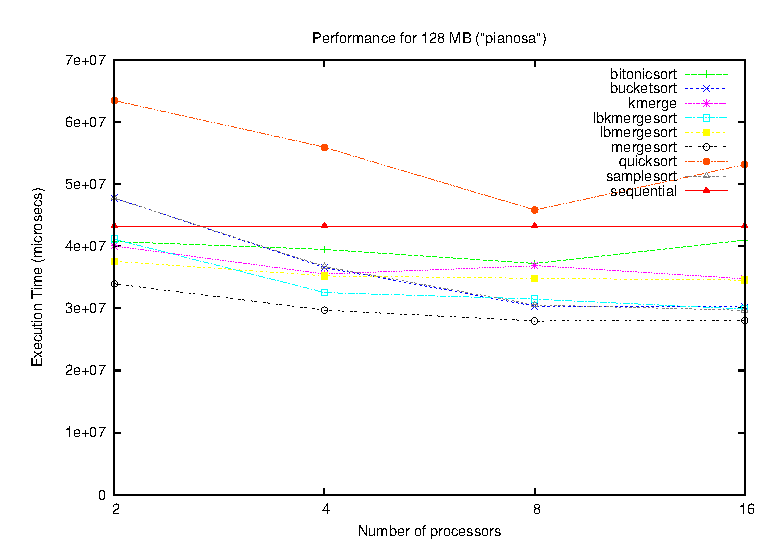
\includegraphics[width=0.4\textwidth]{plots/test_01_pianosa/NxTxA/M33554432_pianosa_NxTxA}} 
  	
	\caption{Time Completion for sorting \textit{large} data sets. Each graphic represents a data set of fixed size, while each shape on a graphic shows the Time Completion of a certain Sorting Algorithm for that data set.}
	\label{NxTxA-large}
\end{figure} 

\begin{figure}[!ht]
	\ContinuedFloat
	\centering
	\subfloat[Data set of 64M integers.]{\label{large-sequential}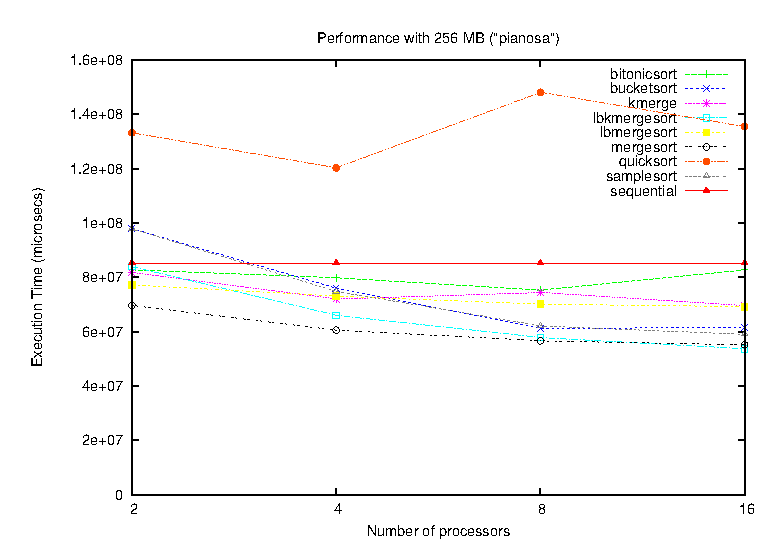
\includegraphics[width=0.4\textwidth]{plots/test_01_pianosa/NxTxA/M67108864_pianosa_NxTxA}} 
	\hspace*{20pt}	
  	\subfloat[Data set of 128M integers.]{\label{large-bitonicsort}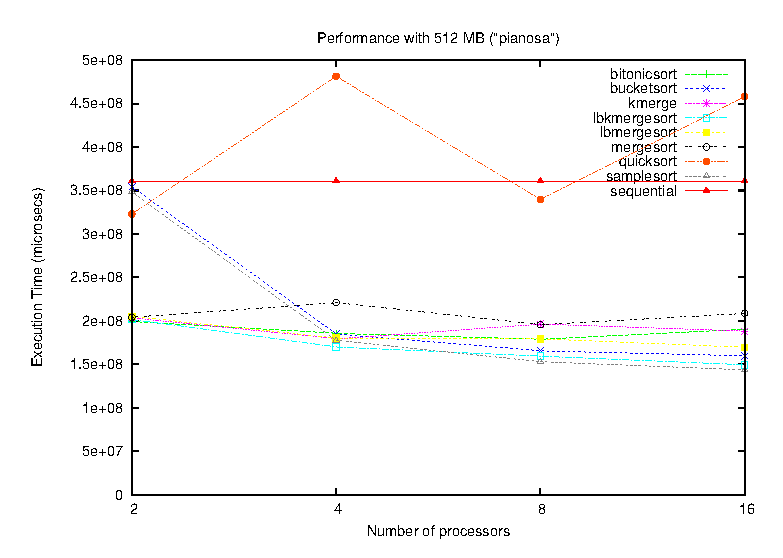
\includegraphics[width=0.4\textwidth]{plots/test_01_pianosa/NxTxA/M134217728_pianosa_NxTxA}} 
  		
	\centering
	\subfloat[Data set of 256M integers.]{\label{large-bucketsort}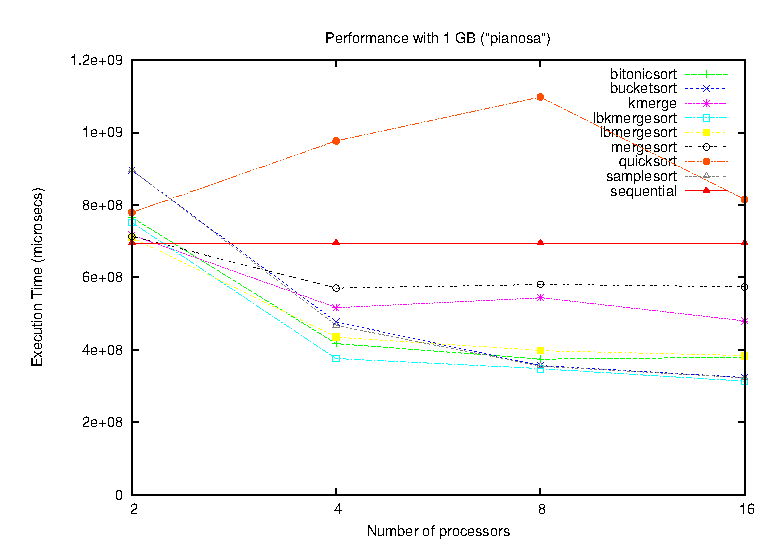
\includegraphics[width=0.4\textwidth]{plots/test_01_pianosa/NxTxA/M268435456_pianosa_NxTxA}} 
  	\hspace*{20pt}
  	\subfloat[Data set of 512M integers.]{\label{large-samplesort}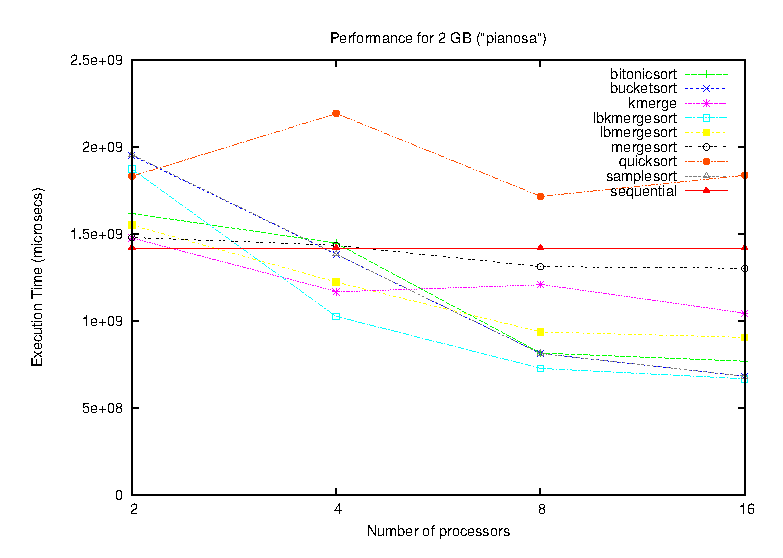
\includegraphics[width=0.4\textwidth]{plots/test_01_pianosa/NxTxA/M536870912_pianosa_NxTxA}} 
	
	\centering
  	\subfloat[Data set of 1G integers.]{\label{large-mergesort}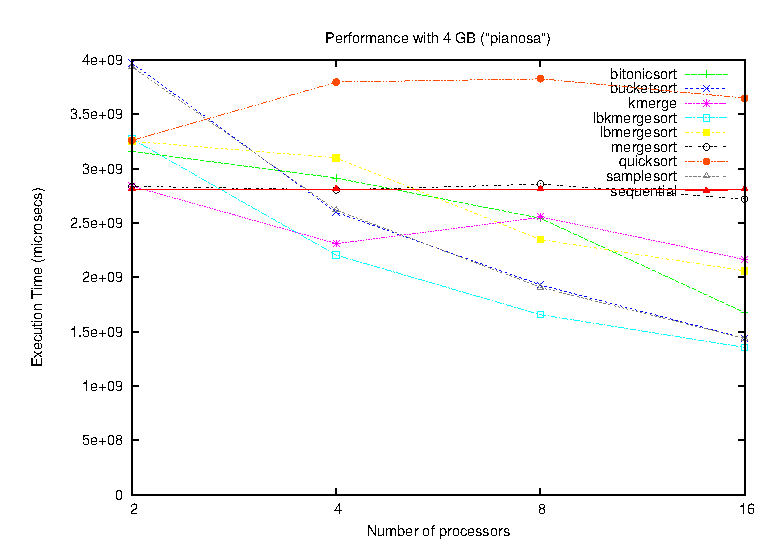
\includegraphics[width=0.4\textwidth]{plots/test_01_pianosa/NxTxA/M1073741824_pianosa_NxTxA}}    
  	
	\caption{Time Completion for sorting \textit{huge} data sets. Each graphic represents a data set of fixed size, while each shape on a graphic shows the Time Completion of a certain Sorting Algorithm for that data set.}
	\label{NxTxA-huge}
\end{figure} 

\begin{figure}[!ht]
	\ContinuedFloat
	\centering
	\subfloat[Parallelism degree 2.]{\label{large-sequential}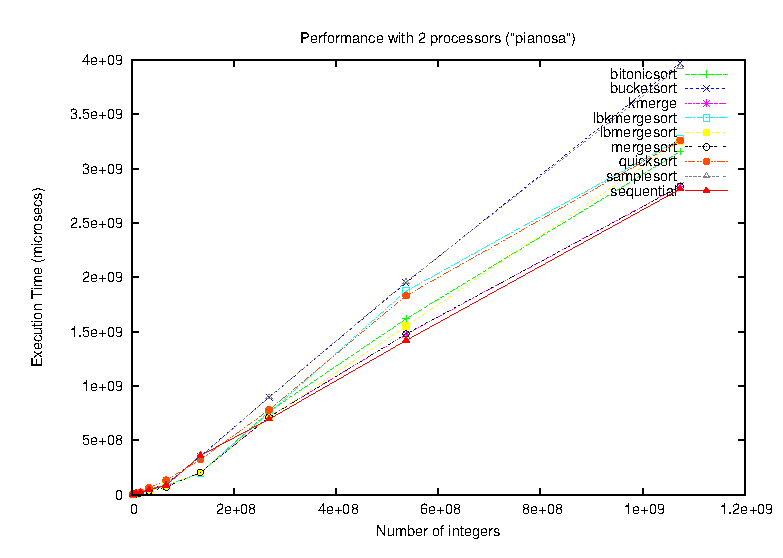
\includegraphics[width=0.4\textwidth]{plots/test_01_pianosa/MxTxA/n2_pianosa_MxTxA}} 
	\hspace*{20pt}	
  	\subfloat[Parallelism degree 4.]{\label{large-bitonicsort}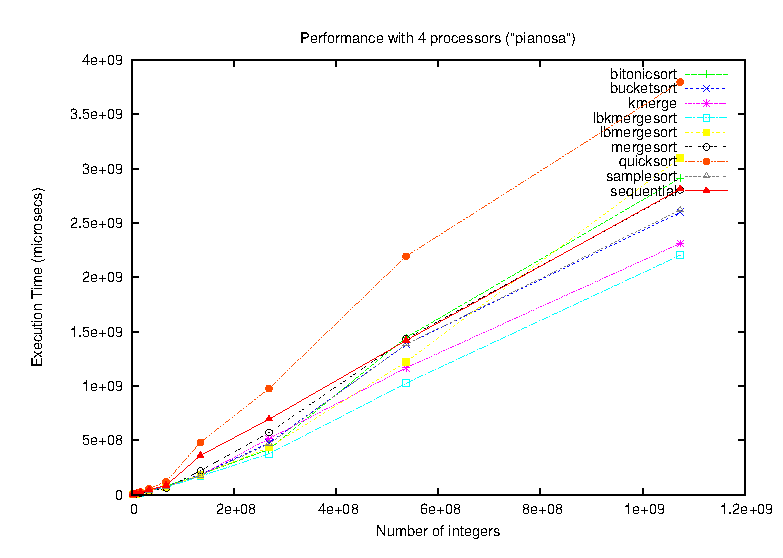
\includegraphics[width=0.4\textwidth]{plots/test_01_pianosa/MxTxA/n4_pianosa_MxTxA}} 
  		
	\centering
	\subfloat[Parallelism degree 8.]{\label{large-bucketsort}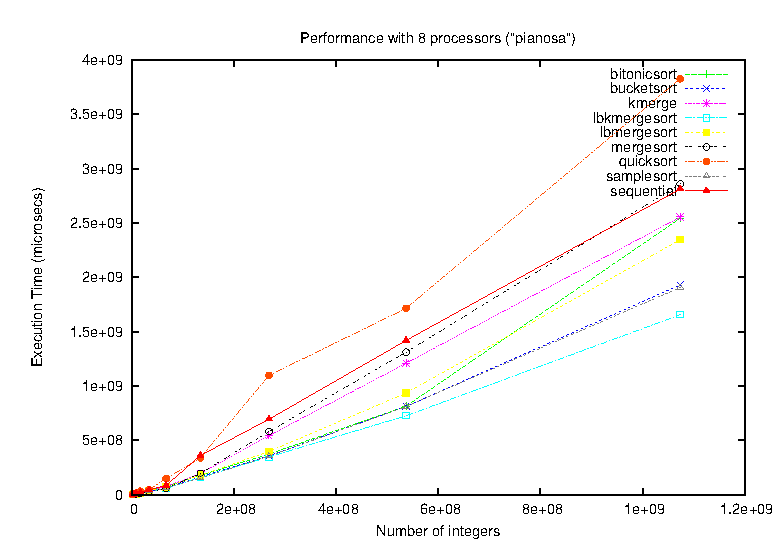
\includegraphics[width=0.4\textwidth]{plots/test_01_pianosa/MxTxA/n8_pianosa_MxTxA}} 
  	\hspace*{20pt}
  	\subfloat[Parallelism degree 16.]{\label{large-samplesort}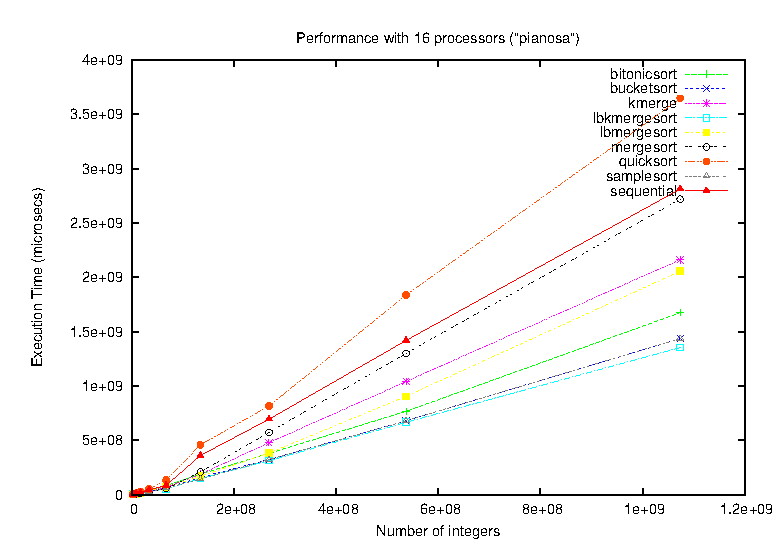
\includegraphics[width=0.4\textwidth]{plots/test_01_pianosa/MxTxA/n16_pianosa_MxTxA}} 
  	
	\caption{Time Completion for sorting data sets with fixed parallelism degree.}
	\label{MxTxA}
\end{figure} 

\clearpage

\subsubsection{Physics}

\paragraph{Scalability of Sorting Algorithms}
\paragraph{Comparison between Sorting Algorithms}
